% main.tex — Curriculum master file (edition-agnostic core)
% -----------------------------------------------------------
% Build editions:
%   latexmk instructor.tex   (or: make instructor)  — includes solutions
%   latexmk student.tex      (or: make student)     — problems + hints only
% Wrappers define \studentmark (student) or \instructormark (instructor)
% BEFORE \input-ing this file.
\newif\ifstudent
\ifdefined\studentmark \studenttrue \fi

\documentclass[11pt,a4paper,openany]{book}

% ---- Foundations (order matters) ---------------------------
\usepackage{xcolor}
% config/colors.tex — Curriculum design system color palette
% -----------------------------------------------------------
% Palette "Oxford Study": muted, print-friendly academic tones.
% All colors are safe for grayscale printing (structure survives
% conversion; only accent hue is lost).
%
% To re-skin an entire curriculum, edit ONLY this file.

% ---- Core text & structure ---------------------------------
\definecolor{ink}{HTML}{1C1B1A}          % body text (near-black, warm)
\definecolor{navy}{HTML}{1F3A5F}         % primary: theorems, headings, links
\definecolor{navymid}{HTML}{3D5A80}      % secondary structure
\definecolor{navylight}{HTML}{EAF0F7}    % pale fill for theorem-family boxes
\definecolor{slate}{HTML}{5B6B7C}        % secondary text, hints, source tags
\definecolor{slatelight}{HTML}{F0F3F6}   % pale fill for remarks/hints
\definecolor{rulegray}{HTML}{C7CDD4}     % hairlines, frames, empty stars

% ---- Semantic accents ---------------------------------------
\definecolor{forest}{HTML}{2E6E4E}       % definitions (green = "grows ideas")
\definecolor{forestlight}{HTML}{ECF4EF}  % definition fill
\definecolor{gold}{HTML}{9A7B2E}         % challenge problems, difficulty stars
\definecolor{goldlight}{HTML}{FAF5E6}    % challenge fill
\definecolor{crimson}{HTML}{9E2B25}      % cautions, common pitfalls
\definecolor{crimsonlight}{HTML}{FBF0EF} % pitfall fill
\definecolor{solutionblue}{HTML}{31456B} % solutions (instructor edition)
\definecolor{solutionlight}{HTML}{F1F4F9}% solution fill

% ---- Hyperlinks ----------------------------------------------
\colorlet{linkcolor}{navy}
\colorlet{citecolor}{forest}
\colorlet{urlcolor}{slate}

\usepackage{etoolbox}
\usepackage{environ}
\usepackage{amsmath}
\usepackage{amssymb}
\usepackage{amsthm}
\usepackage{mathtools}

% ---- Fonts & typography (LuaLaTeX) ---------------------------
\usepackage{fontspec}
\usepackage{unicode-math}
% config/typography.tex — Fonts, math setup, micro-typography
% ------------------------------------------------------------
% Requires LuaLaTeX (fontspec + unicode-math, loaded in main.tex
% BEFORE this file). Loaded after config/colors.tex.

% ---- Font set toggle ----------------------------------------
% pagella : TeX Gyre Pagella + Pagella Math  (warm "olympiad book" look)
% modern  : Latin Modern + LM Math            (classic journal look)
\newif\ifpagellafonts
\pagellafontstrue   % <- flip to \pagellafontsfalse for Latin Modern

\ifpagellafonts
  \setmainfont{TeX Gyre Pagella}[
    Ligatures   = TeX,
    BoldFont    = *-Bold,
    ItalicFont  = *-Italic,
    BoldItalicFont = *-BoldItalic,
  ]
  \setsansfont{TeX Gyre Heros}[
    Scale       = 0.92,
    BoldFont    = *-Bold,
    ItalicFont  = *-Italic,
    BoldItalicFont = *-BoldItalic,
  ]
  \setmonofont{Latin Modern Mono}[Scale=0.88]
  \setmathfont{TeX Gyre Pagella Math}
\else
  \setmainfont{Latin Modern Roman}
  \setsansfont{Latin Modern Sans}[Scale=0.92]
  \setmonofont{Latin Modern Mono}[Scale=0.88]
  \setmathfont{Latin Modern Math}
\fi

% Sans font is reserved for labels, running heads, box titles and
% difficulty badges; body and math stay serif for readability.
\newcommand{\labeltext}[1]{{\sffamily\bfseries\color{navy}#1}}

% ---- Micro-typography ---------------------------------------
% Protrusion + font expansion: subtle but lifts the page a full notch.
\usepackage{microtype}
\microtypesetup{
  protrusion = true,
  expansion  = true,
  factor     = 900,
}

% ---- Spacing conventions ------------------------------------
% A touch more leading than default: long math-heavy paragraphs
% with display equations read better.
\usepackage{setspace}
\setstretch{1.04}

% Display math: slightly tighter spacing around equations than default.
\AtBeginDocument{%
  \setlength{\abovedisplayskip}{6pt plus 2pt minus 3pt}%
  \setlength{\belowdisplayskip}{6pt plus 2pt minus 3pt}%
  \setlength{\abovedisplayshortskip}{3pt plus 1pt}%
  \setlength{\belowdisplayshortskip}{3pt plus 1pt}%
}

% Never let a paragraph start on the same line as a display above it.
\usepackage{parskip}%  -- deliberately NOT activated; this template uses
                     %  classic indentation for dense mathematical prose.
% Paragraph indent + skip tuned for curriculum prose:
\setlength{\parindent}{1.15em}
\setlength{\parskip}{2pt plus 1pt}


% ---- Layout ---------------------------------------------------
% config/layout.tex — Page geometry, headers/footers, sectioning
% ---------------------------------------------------------------
% Loaded after typography + colors.

% ---- Page geometry (print-ready, A4, twoside) ----------------
\usepackage{geometry}
\geometry{
  a4paper,
  twoside,
  inner       = 26mm,   % binding side keeps a little extra
  outer       = 22mm,
  top         = 26mm,
  bottom      = 28mm,
  headheight  = 14pt,
  headsep     = 9mm,
  footskip    = 11mm,
  marginparwidth = 24mm, % room for future marginal notes
  marginparsep = 5mm,
}

% ---- Running heads & folios ----------------------------------
\usepackage{fancyhdr}
\pagestyle{fancy}
\fancyhf{}
% Even (verso): chapter title centered-in-left, folio on left edge.
\fancyhead[LE]{\small\sffamily\color{slate}\nouppercase{\leftmark}}
\fancyhead[RO]{\small\sffamily\color{slate}\nouppercase{\rightmark}}
\fancyfoot[LE]{\small\sffamily\color{navy}\thepage}
\fancyfoot[RO]{\small\sffamily\color{navy}\thepage}
\renewcommand{\headrulewidth}{0.4pt}
\renewcommand{\headrule}{\color{rulegray}\hrule width\headwidth height 0.4pt}
% Chapter-open pages: folio only, no head rule.
\fancypagestyle{plain}{%
  \fancyhf{}%
  \fancyfoot[C]{\small\sffamily\color{navy}\thepage}%
  \renewcommand{\headrulewidth}{0pt}}

% ---- Sectioning hierarchy ------------------------------------
\usepackage{titlesec}
% Chapters: big display number, navy title, hairline rule beneath.
\titleformat{\chapter}[display]
  {\normalfont\sffamily}
  {\color{navymid}\fontsize{30}{30}\selectfont\thechapter}
  {10pt}
  {\color{navy}\fontsize{22}{26}\selectfont\bfseries}
  [\vspace{6pt}{\color{rulegray}\titlerule[0.6pt]}\vspace{4pt}]
\titlespacing*{\chapter}{0pt}{-18pt}{26pt}
% Sections: navy sans bold with breathing room.
\titleformat{\section}
  {\normalfont\large\sffamily\bfseries\color{navy}}
  {\thesection}{0.8em}{}
\titlespacing*{\section}{0pt}{18pt plus 4pt minus 2pt}{7pt plus 2pt}
% Subsections: ink sans bold, smaller.
\titleformat{\subsection}
  {\normalfont\normalsize\sffamily\bfseries\color{ink}}
  {\thesubsection}{0.8em}{}
\titlespacing*{\subsection}{0pt}{13pt plus 3pt minus 2pt}{5pt plus 1pt}

% ---- Table of contents depth ---------------------------------
\setcounter{tocdepth}{1}        % chapters + sections
\setcounter{secnumdepth}{2}

% ---- List spacing (with enumitem, loaded in environments) ----
% Tuned here so lists inside tight boxes stay readable.
\AtBeginDocument{%
  \setlist{topsep=4pt, itemsep=2.5pt, parsep=0pt}%
}


% ---- Graphics & tables -----------------------------------------
\usepackage{tikz}
\usetikzlibrary{shapes.geometric,calc,decorations.pathreplacing}
\usepackage{pgfplots}
\pgfplotsset{compat=1.18}
\usepackage{booktabs}
\usepackage{array}
\usepackage{tabularx}
\usepackage{longtable}
\usepackage{caption}
\captionsetup{font=small, labelfont={bf,color=navy}, skip=6pt}

% ---- Author macros & environments -----------------------------
% config/commands.tex — Author-facing macros: notation, difficulty, tags
% -----------------------------------------------------------------------
% Requires: xcolor, amsmath, amssymb, tikz (shapes.geometric) — all
% loaded in main.tex before this file.

% =====================  Difficulty indicators  =========================
% \difficulty{n} renders n filled stars + (5-n) empty stars, gold.
% Convention: * = routine, ** = standard olympiad, *** = hard,
%             **** = very hard (national team), ***** = IMO P3/P6 level.
\usetikzlibrary{shapes.geometric}
% One inline star; #1 = fill color, #2 = draw color.
\newcommand{\staricon}[2]{%
  \begin{tikzpicture}[baseline=(s.center)]
    \node[star, star points=5, star point ratio=2.3, inner sep=0.85pt,
          fill=#1, draw=#2, line width=0.45pt] (s) {};
  \end{tikzpicture}%
}
\newcommand{\filledstars}[1]{% #1 filled stars remain
  \ifnum#1>0 \staricon{gold}{gold}\expandafter\filledstars\expandafter{\the\numexpr#1-1}\fi
}
\newcommand{\emptystars}[1]{% #1 outline stars remain
  \ifnum#1>0 \staricon{white}{rulegray}\expandafter\emptystars\expandafter{\the\numexpr#1-1}\fi
}
\newcommand{\difficulty}[1]{\filledstars{#1}\emptystars{\numexpr5-#1\relax}}

% Variant for use on colored title bars (e.g. gold challenge bars):
% white filled stars, pale-gold outline stars.
\newcommand{\filledstarsW}[1]{%
  \ifnum#1>0 \staricon{white}{white}\expandafter\filledstarsW\expandafter{\the\numexpr#1-1}\fi
}
\newcommand{\emptystarsW}[1]{%
  \ifnum#1>0 \staricon{white}{gold!45}\expandafter\emptystarsW\expandafter{\the\numexpr#1-1}\fi
}
\newcommand{\difficultywhite}[1]{\filledstarsW{#1}\emptystarsW{\numexpr5-#1\relax}}

% Text difficulty badge for prose: \difficultytext{2} -> "Level 2"
\newcommand{\difficultytext}[1]{\textbf{\color{gold}Level #1}}

% =====================  Problem metadata  ==============================
% \source{...} — right-aligned provenance tag, e.g. \source{IMO 2005, P1}
\newcommand{\source}[1]{\hfill{\small\sffamily\itshape\color{slate}[#1]}\par}

% \points{n} — optional point value tag for assessments.
\newcommand{\points}[1]{\hfill{\small\sffamily\color{slate}(#1~pt)}\par}

% =====================  Number sets  ====================================
\newcommand{\N}{\mathbb{N}}
\newcommand{\Z}{\mathbb{Z}}
\newcommand{\Q}{\mathbb{Q}}
\newcommand{\R}{\mathbb{R}}
\newcommand{\C}{\mathbb{C}}
\newcommand{\Positive}{\R_{>0}}   % strictly positive reals

% =====================  General math shortcuts  ========================
\DeclareMathOperator{\sgn}{sgn}
\newcommand{\abs}[1]{\lvert #1 \rvert}
\newcommand{\norm}[1]{\lVert #1 \rVert}
\newcommand{\floor}[1]{\left\lfloor #1 \right\rfloor}
\newcommand{\ceil}[1]{\left\lceil #1 \right\rceil}
% Display-style fractions and sums for inline use:
\newcommand{\ds}{\displaystyle}
% Standard big operators with canonical limits:
\newcommand{\sumi}{\sum_{i=1}^{n}}
\newcommand{\sumk}{\sum_{k=1}^{n}}
% QED-flavored end-of-proof symbol is provided by amsthm (\qedhere).

% =====================  Curriculum metadata  ===========================
% Overridden per project (see scripts/init-curriculum.sh).
\newcommand{\CurriculumSeries}{Mathematics Olympiad Series}
\newcommand{\CurriculumTitle}{Curriculum Title}
\newcommand{\CurriculumSubtitle}{Subtitle: Volume and Level}
\newcommand{\CurriculumAuthor}{Author Name}
\newcommand{\CurriculumInstitution}{Institution}
\newcommand{\CurriculumDate}{\today}
\newcommand{\CurriculumEdition}{Student Edition}
\newcommand{\CurriculumVersion}{v0.1.0}

\ifstudent\else
  \renewcommand{\CurriculumEdition}{Instructor Edition}
\fi
\usepackage{enumitem}
% config/environments.tex — Theorem family, examples, exercises, boxes
% -----------------------------------------------------------------------
% Requires (loaded in main.tex before this file):
%   amsmath, amsthm, thmtools, tcolorbox, enumitem, environ,
%   config/colors, config/commands
%
% Design language:
%   * Definition family : green edge, pale green wash  ("growing ideas")
%   * Theorem family    : navy edge, pale blue wash    ("core results")
%   * Remarks/strategies: slate frame, faint wash      ("guidance")
%   * Exercises         : slate frame on white         ("your turn")
%   * Challenges        : gold edge, pale gold wash    ("summit")
%   * Solutions         : blue-gray wash (instructor edition only)
% All boxes are BREAKABLE — they split cleanly across pages.

% =====================  tcolorbox base styles  =========================
\usepackage{thmtools}     % \declaretheorem (requires amsthm, already loaded)
\usepackage{tcolorbox}
\tcbuselibrary{skins,breakable,theorems}
\tcbset{
  curriculum/.style={
    enhanced, breakable,
    fonttitle=\sffamily\bfseries\small,
    coltitle=white,
    colback=white,
    boxrule=0.5pt, arc=1.6pt,
    left=9pt, right=9pt, top=7pt, bottom=7pt,
    before skip=13pt plus 2pt, after skip=13pt plus 2pt,
    toptitle=3.5pt, bottomtitle=3pt,
  },
  defbox/.style={curriculum, colframe=forest, colback=forestlight,
    leftrule=2.6pt, rightrule=0.5pt, toprule=0.5pt, bottomrule=0.5pt},
  thmbox/.style={curriculum, colframe=navy, colback=navylight,
    leftrule=2.6pt, rightrule=0.5pt, toprule=0.5pt, bottomrule=0.5pt},
  remarkbox/.style={curriculum, colframe=slate, colback=slatelight,
    boxrule=0.5pt, colbacktitle=slate},
  exbox/.style={curriculum, colframe=slate!75, colback=white,
    boxrule=0.6pt, colbacktitle=slate!75,
    titlerule=0.5pt, titlerule style={slate!45}},
  chalbox/.style={curriculum, colframe=gold, colback=goldlight,
    leftrule=2.6pt, rightrule=0.5pt, toprule=0.5pt, bottomrule=0.5pt},
  solbox/.style={curriculum, colframe=solutionblue!90, colback=solutionlight,
    boxrule=0.5pt, colbacktitle=solutionblue!90},
}

% =====================  Theorem machinery  =============================
% Shared counter across theorem/lemma/proposition/corollary; definitions
% and examples carry their own per-chapter counters.
\declaretheorem[style=plain, name=Theorem, parent=chapter]{theorem}
\declaretheorem[style=plain, name=Lemma, sibling=theorem]{lemma}
\declaretheorem[style=plain, name=Proposition, sibling=theorem]{proposition}
\declaretheorem[style=plain, name=Corollary, sibling=theorem]{corollary}
\declaretheorem[style=definition, name=Definition, parent=chapter]{definition}
\declaretheorem[style=definition, name=Example, parent=chapter]{example}
\declaretheorem[style=remark, name=Remark, numbered=unless unique,
  parent=chapter]{remark}
\declaretheorem[style=remark, name=Key Idea, parent=chapter]{keyidea}
\declaretheorem[style=remark, name=Strategy, parent=chapter]{strategy}
\declaretheorem[style=remark, name=Common Pitfall, parent=chapter]{pitfall}

% Wrap the named environments in their boxes. Proofs stay unboxed
% (amsthm), typeset in the standard way for maximal readability.
\tcolorboxenvironment{theorem}{thmbox}
\tcolorboxenvironment{lemma}{thmbox}
\tcolorboxenvironment{proposition}{thmbox}
\tcolorboxenvironment{corollary}{thmbox}
\tcolorboxenvironment{definition}{defbox}
\tcolorboxenvironment{example}{exbox}
\tcolorboxenvironment{remark}{remarkbox}
\tcolorboxenvironment{keyidea}{remarkbox}
\tcolorboxenvironment{strategy}{remarkbox}
\tcolorboxenvironment{pitfall}{%
  curriculum, colframe=crimson, colback=crimsonlight,
  leftrule=2.6pt, rightrule=0.5pt, toprule=0.5pt, bottomrule=0.5pt,
  colbacktitle=crimson}

% Worked solutions inside examples: proof-like block with custom head.
\newenvironment{exsolution}{\begin{proof}[\normalfont\sffamily\bfseries\color{navy}Solution.]}{\end{proof}}

% =====================  Exercises with difficulty  =====================
% \begin{exercise}{3}                     -> 3-star exercise
% \begin{exercise}[label=ex:mylabel]{3}   -> add \label for solutions
% Optional tcolorbox keys go in the bracketed argument.
\newtcolorbox[auto counter, number within=chapter]{exercise}[2][]{%
  exbox,
  title={Exercise \thetcbcounter\ \hfill \difficulty{#2}},
  breakable, enhanced,
  #1
}

% Challenge problems: gold boxes, separate counter. Stars are the
% white variant: gold stars would vanish on the gold title bar.
\newtcolorbox[auto counter, number within=chapter]{challenge}[2][]{%
  chalbox,
  title={Challenge \thetcbcounter\ \hfill \difficultywhite{#2}},
  breakable, enhanced,
  #1
}

% =====================  Hints & solutions  =============================
% Hint: compact slate box for inline or collected hints.
\newtcolorbox{hint}[1][]{%
  remarkbox, coltitle=white,
  left=7pt, right=7pt, top=5pt, bottom=5pt,
  before skip=9pt, after skip=9pt,
  title={Hint}, #1
}

% Solution: matches a labeled exercise; instructor edition only.
% Usage: \begin{solution}{ex:1-3} ... \end{solution}
\newtcolorbox{solution}[1]{%
  solbox,
  title={Solution to Exercise~\ref{#1}},
}

% =====================  Chapter furniture  =============================
% Learning objectives: opening box with checked items.
\newtcolorbox{objectives}[1][]{%
  thmbox, title={Learning Objectives}, #1
}
% Objective item with gold check bullet (use inside itemize).
\newcommand{\objective}{\item[\textcolor{gold}{$\checkmark$}]}

% Prerequisites: compact slate box.
\newtcolorbox{prerequisites}[1][]{%
  remarkbox, title={Prerequisites}, #1
}

% Notation table box.
\newtcolorbox{notation}[1][]{%
  remarkbox, title={Notation}, #1
}

% Chapter summary: end-of-chapter distilled results.
\newtcolorbox{chaptersummary}[1][]{%
  thmbox, title={Chapter Summary}, #1
}
% Summary item with navy triangle bullet (use inside itemize).
\newcommand{\summaryitem}{\item[\textcolor{navy}{\small$\blacktriangleright$}]}

% =====================  Answer key helper  =============================
% \answer{42} — quick answer line for answer keys.
\newcommand{\answer}[1]{\par\smallskip\noindent\labeltext{Answer:} #1\par}

% =====================  Instructor-only note  ==========================
% Visible only in the instructor edition; absorbed silently otherwise.
\ifstudent
  \NewEnviron{instructornote}{}%
\else
  \newtcolorbox{instructornote}[1][]{%
    remarkbox, colbacktitle=crimson, title={Instructor Note}, #1}
\fi


% ---- Bibliography ---------------------------------------------
\usepackage[numbers,sort&compress]{natbib}
\bibliographystyle{plainnat}
\renewcommand{\bibsection}{\chapter{References and Further Reading}}

% ---- Hyperlinks (near-last) ------------------------------------
\usepackage{hyperref}
\hypersetup{
  colorlinks = true,
  linkcolor  = linkcolor,
  citecolor  = citecolor,
  urlcolor   = urlcolor,
  pdftitle   = {\CurriculumTitle},
  pdfauthor  = {\CurriculumAuthor},
  pdfsubject = {\CurriculumSeries},
  bookmarksnumbered = true,
  bookmarksopen     = true,
  bookmarksopenlevel= 1,
}
\usepackage{bookmark}
\usepackage{cleveref}   % always last
% cleveref names for our custom environments (must follow cleveref load).
\crefname{tcb@cnt@exercise}{Exercise}{Exercises}
\crefname{tcb@cnt@challenge}{Challenge}{Challenges}
\crefname{theorem}{Theorem}{Theorems}
\crefname{lemma}{Lemma}{Lemmas}
\crefname{proposition}{Proposition}{Propositions}
\crefname{corollary}{Corollary}{Corollaries}
\crefname{definition}{Definition}{Definitions}
\crefname{example}{Example}{Examples}
\crefname{keyidea}{Key Idea}{Key Ideas}
\crefname{strategy}{Strategy}{Strategies}
\crefname{pitfall}{Pitfall}{Pitfalls}

% ---- Optional single-chapter builds ---------------------------
% `make chapter C=2` writes <edition>-include.tex, picked up here.
\IfFileExists{\jobname-include.tex}{\input{\jobname-include.tex}}{}

% ===================  DOCUMENT  =================================
\begin{document}

% components/frontmatter.tex — Imprint, preface, TOC
% ----------------------------------------------------
% components/cover.tex — Title page
% -----------------------------------
% Minimal academic cover: series band, title, rule, subtitle, author,
% institution, edition badge. Swap the TikZ motif to re-theme.
\begin{titlepage}
  \thispagestyle{empty}
  \centering
  \vspace*{18mm}

  % Series band
  {\color{navy}\rule{0.62\textwidth}{0.5pt}}\\[6pt]
  {\sffamily\small\bfseries\color{slate}\MakeUppercase{\CurriculumSeries}}\\[3pt]
  {\color{navy}\rule{0.62\textwidth}{0.5pt}}

  \vspace{16mm}

  % Geometric motif: parabola envelope + secant (inequalities theme)
  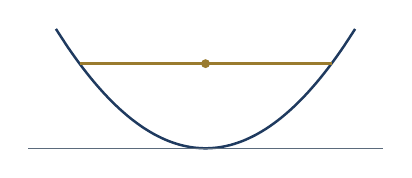
\begin{tikzpicture}[scale=1.0, line width=0.9pt]
    \draw[color=navy,   domain=-1.9:1.9, smooth] plot (\x, {0.42*\x*\x});
    \draw[color=gold]   (-1.6, {0.42*1.6*1.6}) -- (1.6, {0.42*1.6*1.6});
    \fill[color=gold]   (0, {0.42*1.6*1.6}) circle (1.6pt);
    \draw[color=slate,  line width=0.5pt] (-2.25,0) -- (2.25,0);
  \end{tikzpicture}

  \vspace{14mm}

  % Title block
  {\fontsize{30}{34}\selectfont\sffamily\bfseries\color{navy}
    \CurriculumTitle\par}
  \vspace{7mm}
  {\large\itshape\color{slate}\CurriculumSubtitle\par}

  \vspace{18mm}

  % Author & institution
  {\large\CurriculumAuthor\par}
  \vspace{2mm}
  {\normalsize\color{slate}\CurriculumInstitution\par}

  \vfill

  % Edition badge + date
  {\sffamily\small\bfseries\color{white}%
    \tcbox[on line, boxrule=0pt, arc=2pt, left=8pt, right=8pt, top=3.5pt,
           bottom=3.5pt, colback=navy, colframe=navy]
      {\CurriculumEdition}}\par
  \vspace{5mm}
  {\small\color{slate}\CurriculumDate\quad\textbullet\quad\CurriculumVersion\par}

  \vspace{10mm}
\end{titlepage}


% Imprint / edition notes page (verso of cover).
\cleardoublepage
\thispagestyle{empty}
\noindent{\sffamily\bfseries\color{navy}\CurriculumTitle}\\[2pt]
{\small\color{slate}\CurriculumSubtitle\par}
\smallskip
\noindent{\color{rulegray}\rule{\textwidth}{0.4pt}}\par\smallskip
{\small
\noindent\textbf{Edition.} \CurriculumEdition{} (\CurriculumVersion),
compiled \CurriculumDate.\par
\smallskip
\noindent\textbf{About this series.} This volume belongs to the
\CurriculumSeries{}, a structured program of study for competition
mathematics. Each chapter develops theory with complete proofs, worked
examples, and graded problem sets with hints and full solutions.\par
\smallskip
\noindent\textbf{Difficulty scale.}%
\begin{itemize}[leftmargin=1.6em, itemsep=2pt, topsep=3pt]
  \item \difficulty{1}\; Routine reinforcement of a definition or theorem.
  \item \difficulty{2}\; Standard olympiad application; one main idea.
  \item \difficulty{3}\; Hard: requires combining two or more ideas.
  \item \difficulty{4}\; Very hard; shortlist level.
  \item \difficulty{5}\; Olympiad summit (e.g.\ IMO Problem 6 caliber).
\end{itemize}\par}

\frontmatter
\cleardoublepage
\tableofcontents

\cleardoublepage
\section*{Preface}
\markright{Preface}
\noindent This chapter forms the opening unit of the inequalities
strand. It may be read independently; the only background assumed is
fluency with basic algebra and the willingness to check every step of
every proof.

\bigskip
\noindent\textit{How to use this book.} Read each proof actively: cover
it, attempt it, compare. Attempt every exercise before reading its
hint; hints are ordered so that earlier hints spoil less. Full
solutions appear at the end of each chapter.


\mainmatter
% CHAPTERS:BEGIN — scripts/add-chapter.sh inserts \input lines here
% chapters/chapter-01.tex — Inequalities I: AM–GM and Cauchy–Schwarz
% Demonstrates every component of the design system with real content.

\chapter{Inequalities I: \texorpdfstring{AM--GM}{AM-GM} and
         \texorpdfstring{Cauchy--Schwarz}{Cauchy-Schwarz}}
\label{ch:ineq1}

\begin{objectives}
\begin{itemize}
  \objective State and prove the arithmetic--geometric mean inequality
    for two and for $n$ positive reals, including Cauchy's
    forward--backward induction.
  \objective State and prove the Cauchy--Schwarz inequality in two
    ways (discriminant method and Lagrange identity).
  \objective Use the Engel (Titu) form of Cauchy--Schwarz to
    homogenize and crush fraction-sum inequalities.
  \objective Track \emph{equality cases} in every application---the
    difference between an answer and a solution.
\end{itemize}
\end{objectives}

\begin{prerequisites}
\begin{itemize}
  \item Fluency with algebraic manipulation: expanding, factoring,
    completing the square.
  \item Proof by induction (we will extend it in an unusual direction).
  \item Basic sums $\sumi$ notation and its manipulation.
\end{itemize}
\end{prerequisites}

\section{Why Inequalities?}

Exact equalities are the exception in mathematics; controlled
imprecision is the rule. An olympiad inequality problem asks you to
bound one quantity by another, and---crucially---to identify exactly
when the bound is achieved. That second demand is what turns
inequalities from cookbook algebra into proof-writing.

Almost everything in this chapter grows from a single observation:
squares are never negative. From $(a-b)^2 \ge 0$ we will build the
arithmetic--geometric mean inequality (\cref{sec:amgm}), and from a
cleverly chosen quadratic we will build Cauchy--Schwarz
(\cref{sec:cs}). Between them, these two results settle a remarkable
share of competition problems; the classic references are
\cite{steele2004, hlp1952}, and \cite{engel1998} catalogs them by
tactic.

\begin{keyidea}[One source, many rivers]\label{key:source}
Whenever you meet a symmetric inequality in positive variables, ask:
\emph{can I trace it back to a sum of squares?} The three master tools
of this chapter---AM--GM, Cauchy--Schwarz, and the Engel form---are
all squares in disguise.
\end{keyidea}

\section{The Arithmetic--Geometric Mean Inequality}
\label{sec:amgm}

\begin{definition}[Arithmetic and geometric means]\label{def:amgm}
For positive real numbers $a_1, a_2, \dots, a_n$, the
\emph{arithmetic mean} $A$ and \emph{geometric mean} $G$ are
\[
  A \coloneqq \frac{a_1 + a_2 + \cdots + a_n}{n},
  \qquad
  G \coloneqq \sqrt[n]{a_1 a_2 \cdots a_n}.
\]
\end{definition}

We begin with the case $n = 2$, where the entire content is one
perfect square.

\begin{theorem}[AM--GM, two variables]\label{thm:amgm2}
For all positive reals $a, b$,
\[
  \frac{a+b}{2} \;\ge\; \sqrt{ab},
  \qquad\text{with equality if and only if } a = b.
\]
\end{theorem}

\begin{proof}
For any real $t$ we have $(t)^2 \ge 0$. Taking $t = a - b$ and
expanding,
\[
  (a-b)^2 = a^2 - 2ab + b^2 \ge 0
  \quad\Longrightarrow\quad
  a^2 + b^2 \ge 2ab .
\]
Add $2ab$ to both sides:
\[
  a^2 + 2ab + b^2 \ge 4ab
  \quad\Longleftrightarrow\quad
  (a+b)^2 \ge 4ab .
\]
Both sides are positive, so taking square roots preserves the
inequality: $a + b \ge 2\sqrt{ab}$, which is the claim. Equality
forces $(a-b)^2 = 0$, i.e.\ $a = b$.
\end{proof}

\begin{figure}[ht]
  \centering
  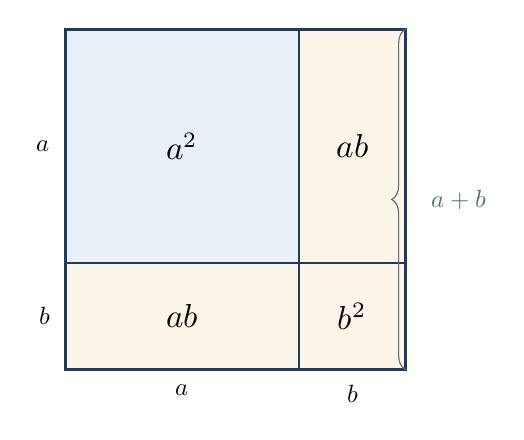
\begin{tikzpicture}[scale=1.35, line cap=round]
    % Square of side a+b (a = 2.2, b = 1.0), split into a 2x2 grid:
    % top-left a^2, top-right ab, bottom-left ab, bottom-right b^2.
    \draw[fill=navylight]  (0,0)   rectangle (2.2,3.2);   % left column
    \draw[fill=goldlight]  (2.2,0) rectangle (3.2,3.2);   % right column
    \draw[fill=goldlight]  (0,0)   rectangle (2.2,1.0);   % bottom-left ab
    \draw[very thick, color=navy] (0,0) rectangle (3.2,3.2);
    % Partition lines: vertical after a=2.2, horizontal after b=1.0.
    \draw[thick, color=navy] (2.2,0) -- (2.2,3.2);
    \draw[thick, color=navy] (0,1.0) -- (3.2,1.0);
    % Area labels
    \node at (1.1,2.1)  {\large $a^2$};
    \node at (2.7,2.1)  {\large $ab$};
    \node at (1.1,0.5)  {\large $ab$};
    \node at (2.7,0.5)  {\large $b^2$};
    % Side length labels
    \node[below=2pt] at (1.1,0) {\small $a$};
    \node[below=2pt] at (2.7,0) {\small $b$};
    \node[left=2pt]  at (0,0.5) {\small $b$};
    \node[left=2pt]  at (0,2.1) {\small $a$};
    % Side brace: total side a+b
    \draw[decorate, decoration={brace, amplitude=5pt}, color=slate]
      (3.2,0) -- (3.2,3.2) node[midway, right=6pt, color=slate] {\small $a+b$};
  \end{tikzpicture}
  \caption{The proof of \cref{thm:amgm2} as geometry. The square of
  side $a+b$ has area $(a+b)^2 = a^2 + 2ab + b^2$; since $a^2 + b^2
  \ge 2ab$ (the two corner squares beat the two $ab$ rectangles in
  total), the area is always at least $4ab$. Equality is the perfectly
  symmetric picture $a = b$, where all four pieces are congruent.}
  \label{fig:amgm-square}
\end{figure}

The general case is one of the most elegant induction arguments in
all of mathematics---\emph{Cauchy's forward--backward induction}. The
statement $P(n)$ is: AM--GM holds for every $n$-tuple of positive
reals. We prove $P(2)$, then $P(n) \Rightarrow P(2n)$ (forward), then
$P(n) \Rightarrow P(n-1)$ (backward). From $P(2)$ we thus get $P(4),
P(8, \dots$ and backward reach \emph{every} integer.

\begin{theorem}[AM--GM, general]\label{thm:amgm}
For all positive reals $a_1, \dots, a_n$,
\[
  \frac{a_1 + \cdots + a_n}{n} \;\ge\; \sqrt[n]{a_1 \cdots a_n},
  \qquad\text{with equality iff } a_1 = \cdots = a_n.
\]
\end{theorem}

\begin{proof}
We follow the plan above.

\emph{Base $P(2)$:} \cref{thm:amgm2}.

\emph{Forward step $P(n) \Rightarrow P(2n)$:} Given $2n$ positive
reals $a_1, \dots, a_{2n}$, split them into two blocks of $n$. Writing
$A_1, G_1$ for the means of the first block and $A_2, G_2$ for the
second, and applying $P(n)$ to each block and then $P(2)$ to the pair
$(A_1, A_2)$:
\[
  \frac{a_1 + \cdots + a_{2n}}{2n}
  = \frac{A_1 + A_2}{2}
  \ge \frac{G_1 + G_2}{2}
  \ge \sqrt{G_1 G_2}
  = \sqrt[2n]{a_1 \cdots a_{2n}} .
\]
Equality forces $A_1 = G_1$, $A_2 = G_2$ (so each block is constant)
and $G_1 = G_2$ (so the constants agree): all $2n$ entries are equal.

\emph{Backward step $P(n) \Rightarrow P(n-1)$:} Given $n - 1$
positive reals $a_1, \dots, a_{n-1}$, let $m$ be their arithmetic
mean and \emph{adjoin the mean itself as an $n$-th entry}. The
enlarged list $a_1, \dots, a_{n-1}, m$ has arithmetic mean
\[
  \frac{(a_1 + \cdots + a_{n-1}) + m}{n}
  = \frac{(n-1)m + m}{n} = m,
\]
so applying $P(n)$ to it yields
\[
  m \;\ge\; \sqrt[n]{a_1 \cdots a_{n-1} \cdot m}
  \quad\Longrightarrow\quad
  m^n \ge a_1 \cdots a_{n-1} \cdot m
  \quad\Longrightarrow\quad
  m^{n-1} \ge a_1 \cdots a_{n-1},
\]
where we divided by $m > 0$. Taking $(n-1)$-th roots gives $m \ge
\sqrt[n-1]{a_1 \cdots a_{n-1}}$, which is $P(n-1)$. Equality in
$P(n)$ forces the enlarged list to be constant; since its last entry
is $m$, the original $n-1$ entries all equal $m$.

Starting from $P(2)$, forward induction gives $P(2^k)$ for all $k$;
for any $n$, choose $k$ with $2^k \ge n$ and descend by the backward
step. \end{proof}

\begin{example}[The workhorse $x + 1/x$]\label{ex:reciprocal}
For every $x > 0$,
\[
  x + \frac{1}{x} \;\ge\; 2\sqrt{x \cdot \tfrac{1}{x}} = 2,
  \qquad\text{equality iff } x = 1 .
\]
\Cref{fig:x-reciprocal} shows why this single line solves many
problems: the function dips to its minimum exactly once, tangentially.
\end{example}

\begin{figure}[ht]
  \centering
  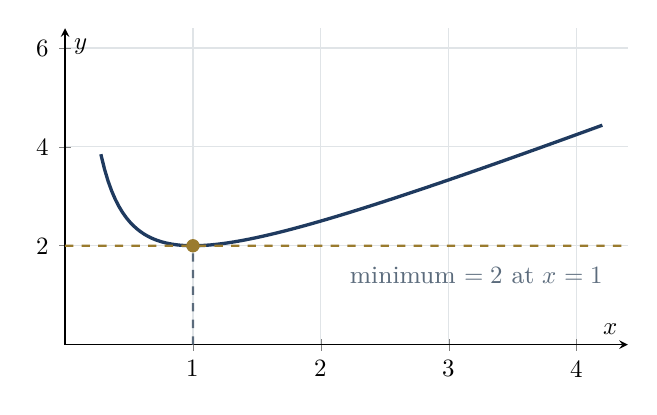
\begin{tikzpicture}
    \begin{axis}[
      width=0.72\textwidth, height=5.6cm,
      axis lines = middle,
      xlabel={$x$}, ylabel={$y$},
      xmin=0, xmax=4.4, ymin=0, ymax=6.4,
      xtick={1,2,3,4}, ytick={2,4,6},
      tick label style={font=\small},
      label style={font=\small},
      grid=both, grid style={rulegray!35},
      major grid style={rulegray!55},
    ]
      \addplot[very thick, color=navy, domain=0.28:4.2, samples=140]
        {x + 1/x};
      \addplot[dashed, color=gold, thick] (0,2) -- (4.4,2);
      \addplot[dashed, color=slate, thick] (1,0) -- (1,2);
      \addplot[only marks, mark=*, mark size=2.2pt, color=gold]
        coordinates {(1,2)};
      \node[font=\small, color=slate, anchor=west] at (axis cs:2.15,1.4)
        {minimum $=2$ at $x=1$};
    \end{axis}
  \end{tikzpicture}
  \caption{$f(x) = x + 1/x$ lies above the line $y = 2$ for all
  $x>0$, touching it only at $x=1$: AM--GM made visible.}
  \label{fig:x-reciprocal}
\end{figure}

\begin{example}[Fixed perimeter, maximal area]\label{ex:perimeter}
Among all rectangles with perimeter $P$, the square has the largest
area.

\begin{exsolution}
Let the side lengths be $a, b > 0$ with $a + b = P/2$. By
\cref{thm:amgm2},
\[
  ab \;\le\; \left(\frac{a+b}{2}\right)^{\!2} = \frac{P^2}{16},
  \qquad\text{equality iff } a = b = \frac{P}{4}.
\]
The maximal area $P^2/16$ is achieved precisely by the square.
\end{exsolution}
\end{example}

\begin{pitfall}[Forgetting the domain]\label{pit:domain}
AM--GM demands \emph{positive} reals. The step $x^2 \le y^2
\Rightarrow x \le y$ used in \cref{thm:amgm2} fails for negative
values, and $\sqrt[n]{\cdot}$ is not even defined (in $\R$) for
negative inputs and even $n$. When a variable can vanish, run AM--GM
on $\varepsilon$-shifted variables or split off the degenerate case.
\end{pitfall}

\section{Cauchy--Schwarz and Its Engel Form}
\label{sec:cs}

\begin{theorem}[Cauchy--Schwarz]\label{thm:cs}
For all real numbers $a_1, \dots, a_n$ and $b_1, \dots, b_n$,
\[
  \left( \sumk a_k b_k \right)^{\!2}
  \;\le\;
  \left( \sumk a_k^2 \right)
  \left( \sumk b_k^2 \right),
\]
with equality iff the vectors $(a_k)$ and $(b_k)$ are proportional.
\end{theorem}

\begin{proof}[First proof (the discriminant trick)]
If all $a_k$ vanish the claim is trivial, so assume
$\sumk a_k^2 > 0$. For every real $t$,
\[
  f(t) \;\coloneqq\; \sumk (a_k t + b_k)^2
  = \Big(\sumk a_k^2\Big) t^2
  + 2\Big(\sumk a_k b_k\Big) t
  + \sumk b_k^2
  \;\ge\; 0,
\]
being a sum of squares. Thus the quadratic $f$ never dips below zero,
so its discriminant is at most $0$:
\[
  \Delta = 4\left(\sumk a_k b_k\right)^{\!2}
  - 4\left(\sumk a_k^2\right)\left(\sumk b_k^2\right) \le 0,
\]
which rearranges to the claim. Equality means $f$ has a real double
root $t_0$: then $a_k t_0 + b_k = 0$ for every $k$, i.e.\ the vectors
are proportional.
\end{proof}

\begin{proof}[Second proof (Lagrange identity)]
Expanding the right-hand side minus the left:
\[
  \left(\sumk a_k^2\right)\!\left(\sumk b_k^2\right)
  - \left(\sumk a_k b_k\right)^{\!2}
  = \sum_{1 \le i < j \le n} \left( a_i b_j - a_j b_i \right)^2 \!\ge 0 .
\]
Every summand on the right is a square. Equality forces
$a_i b_j = a_j b_i$ for all pairs $i<j$, which for nonzero vectors
says exactly: proportional.
\end{proof}

\begin{corollary}[Engel form / Titu's lemma]\label{cor:engel}
For positive reals $b_1, \dots, b_n$ and arbitrary reals
$a_1, \dots, a_n$,
\[
  \sumk \frac{a_k^2}{b_k}
  \;\ge\;
  \frac{(a_1 + \cdots + a_n)^2}{b_1 + \cdots + b_n},
\]
with equality iff the ratios $a_k / b_k$ are all equal.
\end{corollary}

\begin{proof}
Apply \cref{thm:cs} to the vectors
$\big(a_1/\sqrt{b_1}, \dots, a_n/\sqrt{b_n}\big)$ and
$\big(\sqrt{b_1}, \dots, \sqrt{b_n}\big)$:
\[
  (a_1 + \cdots + a_n)^2
  = \left(\sumk \frac{a_k}{\sqrt{b_k}} \cdot \sqrt{b_k}\right)^{\!2}
  \le \left(\sumk \frac{a_k^2}{b_k}\right)
       \left(\sumk b_k\right). \qedhere
\]
\end{proof}

The Engel form turns sums of fractions into one fraction---a
\emph{homogenizing} move of enormous competitive value.

\begin{example}[Nesbitt's inequality]\label{ex:nesbitt}
For $a, b, c > 0$,
\[
  \frac{a}{b+c} + \frac{b}{c+a} + \frac{c}{a+b} \;\ge\; \frac{3}{2}.
\]

\begin{exsolution}
Write each term with a square on top,
$\dfrac{a}{b+c} = \dfrac{a^2}{ab+ac}$, and apply \cref{cor:engel} to
the three fractions:
\[
  \frac{a^2}{ab+ac} + \frac{b^2}{bc+ba} + \frac{c^2}{ca+cb}
  \;\ge\;
  \frac{(a+b+c)^2}{2(ab+bc+ca)} .
\]
Now $(a+b+c)^2 \ge 3(ab+bc+ca)$, because the difference is
$\tfrac{1}{2}\big[(a-b)^2 + (b-c)^2 + (c-a)^2\big] \ge 0$. Hence the
right side is at least
$\tfrac{3(ab+bc+ca)}{2(ab+bc+ca)} = \tfrac{3}{2}$. Equality holds
exactly at $a = b = c$.
\end{exsolution}
\end{example}

\begin{strategy}[The Engel playbook]\label{str:engel}
When a target inequality involves $\sum \frac{(\text{something})^2}
{\text{something}}$---or can be massaged into that shape:
\begin{enumerate}[label=\arabic*., itemsep=2pt]
  \item force a square into each numerator
        ($\frac{a}{b+c} \mapsto \frac{a^2}{ab+ac}$);
  \item apply \cref{cor:engel} to collapse the sum to one fraction;
  \item clean up with whatever symmetric bound remains
        (often $(a+b+c)^2 \ge 3(ab+bc+ca)$);
  \item \emph{verify the equality case} before declaring victory.
\end{enumerate}
Many further worked examples of this playbook appear in
\cite{andreescu2000, kedlaya1999}.
\end{strategy}

\ifstudent\else
\begin{instructornote}
When teaching \cref{ex:nesbitt}, resist writing the Engel application
immediately. First let students try common denominators and watch the
combinatorial explosion---the motivation for homogenization lands much
harder after twenty seconds of suffering.
\end{instructornote}
\fi

\section{Problems}
\label{sec:problems-1}

\noindent Difficulty is marked on the five-star scale explained in the
front matter. Attempt each problem before reading its hint.

% exercises/problems-01.tex — Problems for Chapter 1
% Usage: \begin{exercise}[label=ex:1-N]{difficulty}
%        difficulty: 1=* routine ... 5=***** IMO P6 caliber

\begin{exercise}[label=ex:1-1]{1}
Prove that for all $x > 0$,
\[
  x + \frac{4}{x} \;\ge\; 4,
\]
and determine exactly when equality holds.
\end{exercise}

\begin{exercise}[label=ex:1-2]{1}
Prove that for all $a, b > 0$,
\[
  (a + b)\left( \frac{1}{a} + \frac{1}{b} \right) \ge 4 .
\]
\end{exercise}

\begin{exercise}[label=ex:1-3]{2}
Let $a, b, c$ be real numbers with $a + b + c = 1$. Prove that
\[
  a^2 + b^2 + c^2 \;\ge\; \frac{1}{3}.
\]
\end{exercise}

\begin{exercise}[label=ex:1-4]{2}
Prove that for all real $a, b, c$,
\[
  a^2 + b^2 + c^2 \;\ge\; ab + bc + ca .
\]
\end{exercise}

\begin{exercise}[label=ex:1-5]{2}
Let $x, y, z$ be positive reals with $xyz = 1$. Prove that
\[
  x + y + z \;\ge\; 3 .
\]
\end{exercise}

\begin{exercise}[label=ex:1-6]{3}
Let $x, y, z$ be positive reals. Prove that
\[
  (x + y)(y + z)(z + x) \;\ge\; 8xyz .
\]
\end{exercise}

\begin{exercise}[label=ex:1-7]{3}
Let $a, b, c$ be nonnegative reals with $a + b + c = 6$. Find the
maximum value of $\sqrt{a} + \sqrt{b} + \sqrt{c}$ and all triples
attaining it.
\end{exercise}

\begin{exercise}[label=ex:1-8]{3}
Let $x, y, z$ be positive reals. Prove that
\[
  \frac{x^2}{y+z} + \frac{y^2}{z+x} + \frac{z^2}{x+y}
  \;\ge\; \frac{x+y+z}{2}.
\]
\end{exercise}

\begin{challenge}[label=ch:1-1]{4}
Let $a, b, c$ be positive reals. Prove that
\[
  \frac{a^3}{a^2 + ab + b^2}
  + \frac{b^3}{b^2 + bc + c^2}
  + \frac{c^3}{c^2 + ca + a^2}
  \;\ge\; \frac{a+b+c}{3}.
\]
\source{Training problem (Shapiro--type)}
\end{challenge}

\begin{challenge}[label=ch:1-2]{5}
Let $a, b, c$ be positive reals. Prove that
\[
  \frac{a}{\sqrt{a^2 + 8bc}}
  + \frac{b}{\sqrt{b^2 + 8ca}}
  + \frac{c}{\sqrt{c^2 + 8ab}}
  \;\ge\; 1 .
\]
\source{IMO 2001, Problem 2}
\end{challenge}


\section{Hints}
\label{sec:hints-1}

% exercises/hints-01.tex — Hints for Chapter 1 problems
% Convention: one hint per problem, escalating specificity. Numbering
% matches the exercise counter; challenges are prefixed C.

\begin{itemize}[leftmargin=2.2em, itemsep=5pt, label={}]
  \item[\textbf{1.}] Direct AM--GM on the pair $\big(x, \tfrac{4}{x}\big)$.
    What is the product of the two terms?
  \item[\textbf{2.}] Expand, then pair each fraction with its
    reciprocal twin: $\tfrac{a}{b} + \tfrac{b}{a} \ge 2$.
  \item[\textbf{3.}] Cauchy--Schwarz with
    $(1, 1, 1) \cdot (a, b, c)$: bound $(a+b+c)^2$ from above by
    $3(a^2+b^2+c^2)$.
  \item[\textbf{4.}] Multiply the desired inequality by $2$ and
    recognize three perfect squares.
  \item[\textbf{5.}] AM--GM on three terms; the constraint $xyz = 1$
    makes the geometric mean equal to $1$.
  \item[\textbf{6.}] Bound each factor separately by AM--GM, then
    multiply the three bounds.
  \item[\textbf{7.}] Cauchy--Schwarz on
    $(\sqrt a + \sqrt b + \sqrt c)^2$; equality analysis will
    identify the maximizer.
  \item[\textbf{8.}] Engel form (\cref{cor:engel}) collapses the
    three fractions; the denominator becomes $2(x+y+z)$.
  \item[\textbf{C1.}] Prove the pointwise bound
    $\dfrac{a^3}{a^2+ab+b^2} \ge \dfrac{2a-b}{3}$
    by clearing denominators, then sum.
  \item[\textbf{C2.}] Engel form rewrites the left side as
    $\sum \frac{a^2}{a\sqrt{a^2+8bc}}$. Then Cauchy--Schwarz once
    more, expand $(a+b+c)^3$, and finish with six-term AM--GM.
\end{itemize}


\ifstudent\else
\section{Solutions}
\label{sec:solutions-1}
% exercises/solutions-01.tex — Full solutions for Chapter 1
% Rendered in the instructor edition only (guarded in the chapter).

% ---------- Exercise 1.1 -------------------------------------------------
\begin{solution}{ex:1-1}
Apply AM--GM (\cref{thm:amgm2}) to the pair
$\big(x, \tfrac{4}{x}\big)$, whose product is $4$:
\[
  x + \frac{4}{x} \;\ge\; 2\sqrt{x \cdot \frac{4}{x}} = 2\sqrt4 = 4 .
\]
Equality holds iff $x = \tfrac{4}{x}$, i.e.\ $x = 2$.
\answer{$x + 4/x = 4$ exactly at $x = 2$.}
\end{solution}

% ---------- Exercise 1.2 -------------------------------------------------
\begin{solution}{ex:1-2}
Expanding,
\[
  (a+b)\left(\frac1a + \frac1b\right)
  = 1 + \frac{a}{b} + \frac{b}{a} + 1
  = 2 + \frac{a}{b} + \frac{b}{a}.
\]
By AM--GM on the pair $\big(\tfrac{a}{b}, \tfrac{b}{a}\big)$, whose
product is $1$,
\[
  \frac{a}{b} + \frac{b}{a} \ge 2 ,
\]
so the original expression is at least $4$. Equality holds iff
$\tfrac{a}{b} = \tfrac{b}{a}$, i.e.\ $a = b$.
\end{solution}

% ---------- Exercise 1.3 -------------------------------------------------
\begin{solution}{ex:1-3}
By Cauchy--Schwarz (\cref{thm:cs}) applied to $(1,1,1)$ and
$(a,b,c)$,
\[
  (a+b+c)^2 \;\le\; 3\,(a^2+b^2+c^2).
\]
Since $a+b+c = 1$, this gives $a^2+b^2+c^2 \ge \tfrac13$. Equality
holds iff $(a,b,c)$ is proportional to $(1,1,1)$, i.e.\
$a=b=c=\tfrac13$.
\end{solution}

% ---------- Exercise 1.4 -------------------------------------------------
\begin{solution}{ex:1-4}
Multiply the target by $2$ and rearrange:
\[
  2(a^2+b^2+c^2) - 2(ab+bc+ca)
  = (a-b)^2 + (b-c)^2 + (c-a)^2 \;\ge\; 0,
\]
a sum of squares. Equality holds iff $a = b = c$. Note this is
exactly the identity used in \cref{ex:nesbitt}.
\end{solution}

% ---------- Exercise 1.5 -------------------------------------------------
\begin{solution}{ex:1-5}
By AM--GM for three variables (\cref{thm:amgm}, $n=3$),
\[
  \frac{x+y+z}{3} \;\ge\; \sqrt[3]{xyz} = \sqrt[3]{1} = 1,
\]
so $x+y+z \ge 3$. Equality holds iff $x=y=z=1$.
\end{solution}

% ---------- Exercise 1.6 -------------------------------------------------
\begin{solution}{ex:1-6}
Apply \cref{thm:amgm2} to each factor:
\[
  x+y \ge 2\sqrt{xy}, \qquad
  y+z \ge 2\sqrt{yz}, \qquad
  z+x \ge 2\sqrt{zx}.
\]
All three left sides are positive, so multiplying the inequalities is
legitimate:
\[
  (x+y)(y+z)(z+x) \;\ge\; 8\sqrt{xy \cdot yz \cdot zx}
  = 8\sqrt{x^2y^2z^2} = 8xyz .
\]
Equality holds iff $x=y=z$.
\end{solution}

% ---------- Exercise 1.7 -------------------------------------------------
\begin{solution}{ex:1-7}
By Cauchy--Schwarz applied to
$(\sqrt a, \sqrt b, \sqrt c)$ and $(1,1,1)$,
\[
  (\sqrt a + \sqrt b + \sqrt c)^2
  \;\le\; 3\,(a+b+c) = 18,
\]
so $\sqrt a + \sqrt b + \sqrt c \le 3\sqrt2$.
\answer{Maximum $= 3\sqrt2$, attained only at $(a,b,c) = (2,2,2)$.}
Equality in Cauchy--Schwarz requires
$(\sqrt a, \sqrt b, \sqrt c)$ proportional to $(1,1,1)$, i.e.\
$a=b=c$; combined with $a+b+c=6$ this forces $a=b=c=2$, which
indeed gives $3\sqrt2$. Since the domain $\{a,b,c \ge 0,\;
a+b+c=6\}$ is compact and the objective is continuous, the maximum
exists, so the bound is sharp.
\end{solution}

% ---------- Exercise 1.8 -------------------------------------------------
\begin{solution}{ex:1-8}
Apply the Engel form (\cref{cor:engel}) to the three fractions:
\[
  \frac{x^2}{y+z} + \frac{y^2}{z+x} + \frac{z^2}{x+y}
  \;\ge\;
  \frac{(x+y+z)^2}{(y+z)+(z+x)+(x+y)}
  = \frac{(x+y+z)^2}{2(x+y+z)}
  = \frac{x+y+z}{2} .
\]
Equality holds iff $\tfrac{x}{y+z} = \tfrac{y}{z+x} = \tfrac{z}{x+y}$,
which (cross-multiplying and subtracting) forces $x=y=z$.
\end{solution}

% ---------- Challenge 1 ---------------------------------------------------
\begin{solution}{ch:1-1}
Following the hint, we prove the pointwise bound
\[
  \frac{a^3}{a^2+ab+b^2} \;\ge\; \frac{2a-b}{3} .
\]
Since $a^2+ab+b^2 > 0$, clearing denominators shows the difference is
\[
  3a^3 - (2a-b)(a^2+ab+b^2)
  \;=\; 3a^3 - \big(2a^3 + a^2b + ab^2 - b^3\big)
  \;=\; (a+b)(a-b)^2 \;\ge\; 0,
\]
where the factorization is verified by expanding
$(a+b)(a-b)^2 = a^3 - a^2b - ab^2 + b^3$. Equality holds iff $a=b$.
Applying the same bound to the other two cyclic terms and summing,
\[
  \sum_{\text{cyc}} \frac{a^3}{a^2+ab+b^2}
  \;\ge\;
  \frac{(2a-b) + (2b-c) + (2c-a)}{3}
  = \frac{a+b+c}{3} .
\]
Equality requires $a=b$, $b=c$, and $c=a$ simultaneously---that is,
$a=b=c$, where both sides indeed agree (each fraction equals
$\tfrac{a}{3}$).
\end{solution}

% ---------- Challenge 2 (IMO 2001/2) --------------------------------------
\begin{solution}{ch:1-2}
Write $S = a+b+c$. We chain three estimates.

\emph{Step 1 (Engel).} Writing each term as a square over a product,
\[
  \sum_{\text{cyc}} \frac{a}{\sqrt{a^2+8bc}}
  = \sum_{\text{cyc}} \frac{a^2}{a\sqrt{a^2+8bc}}
  \;\ge\; \frac{S^2}{\displaystyle\sum_{\text{cyc}} a\sqrt{a^2+8bc}}
  \;\eqqcolon\; \frac{S^2}{T},
\]
by \cref{cor:engel} applied with numerators $a$ and denominators
$b = a\sqrt{a^2+8bc}$.

\emph{Step 2 (Cauchy--Schwarz).} Apply \cref{thm:cs} to the vectors
$\big(\sqrt a\big)$ and $\big(\sqrt{a\,(a^2+8bc)}\big)$:
\[
  T^2
  = \left(\sum_{\text{cyc}} \sqrt{a} \cdot
      \sqrt{a(a^2+8bc)}\right)^{\!2}
  \le S \cdot \left(a^3+b^3+c^3 + 24abc\right).
\]

\emph{Step 3 (expansion + AM--GM).} We claim
\[
  a^3+b^3+c^3+24abc \;\le\; S^3 .
\]
Expanding,
\[
  S^3 = a^3+b^3+c^3
  + 3\!\!\sum_{\text{sym}}\! a^2b \; + 6abc,
\]
where $\sum_{\text{sym}} a^2b = a^2b + a^2c + ab^2 + b^2c + ac^2 +
bc^2$. It remains to show $18abc \le 3\sum_{\text{sym}} a^2b$, i.e.\
$6abc \le \sum_{\text{sym}} a^2b$. This is AM--GM
(\cref{thm:amgm}) applied to the \emph{six} terms of the symmetric
sum: their product is
\[
  (a^2b)(a^2c)(ab^2)(b^2c)(ac^2)(bc^2) = a^6 b^6 c^6,
\]
so their geometric mean is $abc$ and their sum is at least $6abc$.

\emph{Conclusion.} Combining,
\[
  T \le \sqrt{S \cdot S^3} = S^2
  \qquad\Longrightarrow\qquad
  \sum_{\text{cyc}} \frac{a}{\sqrt{a^2+8bc}}
  \;\ge\; \frac{S^2}{T} \ge \frac{S^2}{S^2} = 1 .
\]
Equality in every step requires $a=b=c$: then each term equals
$\tfrac{a}{\sqrt{9a^2}} = \tfrac13$ and the sum is exactly $1$.
\end{solution}

\fi

% components/chapter-summary.tex — End-of-chapter distillation
% Reusable pattern: a chaptersummary box with \summaryitem bullets.
\begin{chaptersummary}
\begin{itemize}
  \summaryitem \textbf{AM--GM (\cref{thm:amgm2}, \cref{thm:amgm}).}
    $\dfrac{a_1 + \cdots + a_n}{n} \ge \sqrt[n]{a_1 \cdots a_n}$ for
    positive reals; equality iff all entries are equal. Proved by
    Cauchy's forward--backward induction: $P(2)$, $P(n) \Rightarrow
    P(2n)$, $P(n) \Rightarrow P(n{-}1)$.
  \summaryitem \textbf{Cauchy--Schwarz (\cref{thm:cs}).}
    $\big(\sum a_kb_k\big)^2 \le \big(\sum a_k^2\big)\big(\sum
    b_k^2\big)$; equality iff the vectors are proportional. Two
    proofs: the discriminant trick on $\sum (a_kt + b_k)^2 \ge 0$,
    and the Lagrange identity
    $\sum_{i<j}(a_ib_j - a_jb_i)^2$.
  \summaryitem \textbf{Engel form (\cref{cor:engel}).}
    $\sum \dfrac{a_k^2}{b_k} \ge \dfrac{(\sum a_k)^2}{\sum b_k}$ for
    $b_k > 0$: the homogenizing workhorse for fraction sums
    (\cref{str:engel}).
  \summaryitem \textbf{The equality case is the problem.} Every
    application above pins down \emph{when} equality holds; a
    solution without this analysis is incomplete.
\end{itemize}
\end{chaptersummary}

\begin{notation}
\begin{tabular}{@{}ll@{}}
  $\Positive$ & strictly positive reals \\
  $\sumk$ & $\sum_{k=1}^{n}$ \\
  $\sum_{\text{sym}} a^2b$ & $a^2b + a^2c + ab^2 + b^2c + ac^2 + bc^2$ \\
  $\sum_{\text{cyc}} f(a,b,c)$ & $f(a,b,c) + f(b,c,a) + f(c,a,b)$ \\
\end{tabular}
\end{notation}


% CHAPTERS:END

\ifstudent
  \backmatter
  \chapter*{About the Solutions}
  \addcontentsline{toc}{chapter}{About the Solutions}
  Complete solutions to all exercises and challenges in this volume are
  published separately in the companion \emph{Instructor Edition}.
  Hints for every problem appear at the end of each chapter---try the
  problem first; hints are ordered so that earlier hints spoil less.
\fi

% Bibliography
\bibliography{references/bibliography}

\end{document}
